\documentclass[border=5pt]{standalone}
\usepackage{tikz}
\usepackage{pgfplots}
\pgfplotsset{compat=1.18}
\pagecolor{white}  % Add this line

\begin{document}
	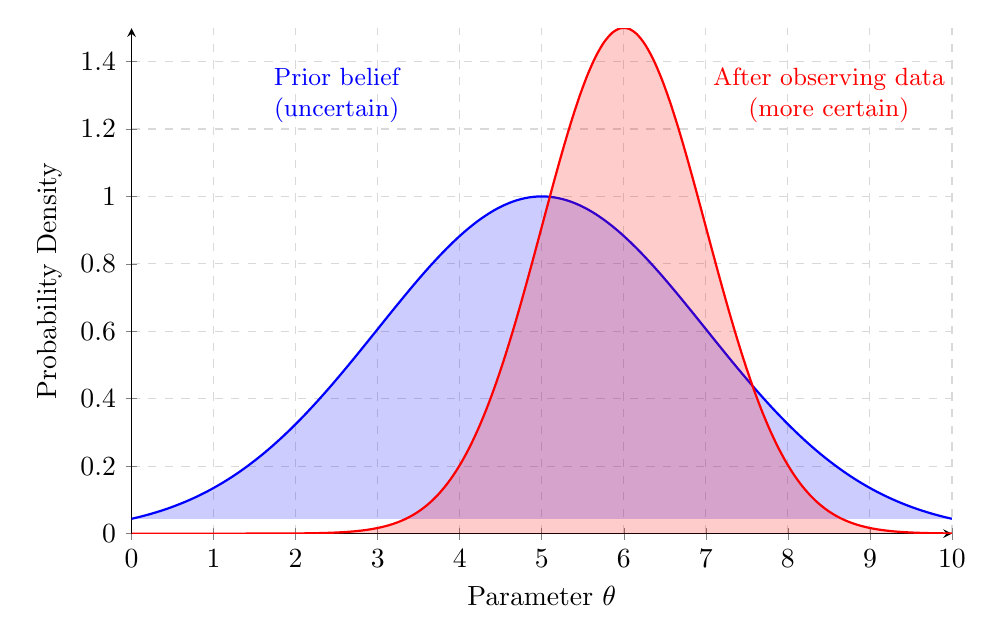
\begin{tikzpicture}
		\begin{axis}[
			width=12cm,
			height=8cm,
			xlabel={Parameter $\theta$},
			ylabel={Probability Density},
			domain=0:10,
			samples=100,
			smooth,
			axis lines=left,
			enlargelimits=false,
			legend pos=north west,
			legend style={fill=white, fill opacity=0.8, draw opacity=1, text opacity=1},
			grid=major,
			grid style={dashed, gray!30},
			]
			
			% Prior distribution (wider, less certain)
			\addplot[
			thick,
			blue,
			fill=blue,
			fill opacity=0.2,
			] {exp(-((x-5)^2)/8)} node[pos=0.3, above, blue] {};
			
			% Posterior distribution (narrower, more certain)
			\addplot[
			thick,
			red,
			fill=red,
			fill opacity=0.2,
			] {1.5*exp(-((x-6)^2)/2)} node[pos=0.5, above, red] {};
			
			%\legend{Prior $p(\theta)$, Posterior $p(\theta|D)$}
			
			% Add annotation
			\node[align=center, font=\small] at (axis cs:2.5,1.3) {
				\textcolor{blue}{Prior belief}\\
				\textcolor{blue}{(uncertain)}
			};
			
			\node[align=center, font=\small] at (axis cs:8.5,1.3) {
				\textcolor{red}{After observing data}\\
				\textcolor{red}{(more certain)}
			};
			
		\end{axis}
	\end{tikzpicture}
\end{document}